\documentclass[MPSI]{cours}
\usepackage{wrapfig}
\usepackage{pgfplots}
\begin{document}
\setcounter{chapter}{27}
\chapter{Introduction à la physique quantique}
\section{La théorie quantique}
\subsection{\'Etat de la physique en 1900}
La physique a considérablement progressé au 18$^e$ et 19$^{e}$ siècles, notamment grâce aux théories de Newton (18$^{e}$) et à Maxwell (19$^e$) qui ont établi les lois de la mécanique, de la gravitation et de l'électromagnétisme. Elles permettent d'expliquer la \emph{quasi-totalité} des phénomènes observés.

\subsection{L'avénement de la physique quantique}
En 1900 il reste quelques phénomènes inexpliqués :

\vspace{1em}
\textbf{La stabilité de l'électron autour du noyau d'un atome} \\
\begin{wrapfigure}{r}{3cm}
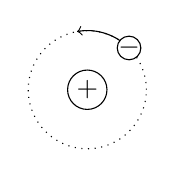
\begin{tikzpicture}[scale=0.5,baseline=(p.base)]
\draw (0,0) circle (0.5cm) node (p) {$+$};
\draw[dotted] (0,0) circle (1.5cm);
\draw[->] (45:1.5cm) arc (45:100:1.5cm);
\draw[fill=white] (45:1.5cm) circle (0.3) node {$-$}; 
\end{tikzpicture}
\end{wrapfigure}
L'électron $-$ tourne autour du noyau $+$ donc il accélère. Maxwell a montré qu'une charge qui accélère rayonne une onde et donc perd de l'énergie.

\textbf{questions :}
\begin{itemize}
\item Pourquoi n'observe-t-on pas de rayonnement ?
\item Pourquoi l'électron ne s'écrase-t-il pas sur le noyau ?
\end{itemize} 

\vspace{2em}
\textbf{Effet photo-électrique (1883)} (Heinrich Hertz 1857-1894)

\begin{center}
\begin{tikzpicture}
\draw (0.5,1) rectangle (0,-1);
\draw (0.25,-1) node[below,align=center] {plaque de \\ métal (Zn)};
\draw[photon] (2,1) node[right,align=left] {lumière de \\ fréquence $\nu$} -- (1,0.6);
\draw (1,-0.5) node {$-$} circle (0.15);
\draw[->] (1,-0.5) ++ (-25:0.2) --++ (-25:0.7) node[right] {électron émis};
\end{tikzpicture}
\end{center}
Lorsqu'on éclaire un métal, dans certaines conditions des électrons sont émispar la surface éclairée.

\textbf{Interprétation :} La lumière transfert son énergie aux électrons qui peuvent alors échapper au métal.

\textbf{problème :} Il existe une fréquence \emph{seuil} $\nu_{lim}$ en dessous de laquelle aucun électron n'est émis :
\begin{center}
  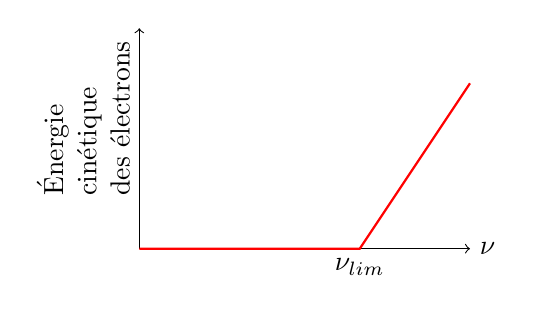
\begin{tikzpicture}[scale=1.4]
\draw[->] (0,0) -- (3,0) node[right] {$\nu$};
\draw[->] (0,0) -- (0,2) node[above left,text width=2cm,rotate=90] {\'Energie cinétique des électrons};
\draw[thick,red] (0,0) -- (2,0) node[below,black] {$\nu_{lim}$} -- (3,1.5);  
\end{tikzpicture}
\end{center}
Au-delà de $\nu_{lim}$, l'énergie cinétique des électrons est 
\begin{equation*}
E_c=h\nu-W
\end{equation*}
$h\simeq\SI{6.63e-34}{Js}$ : Constante de Planck.\\
$W$ : Constante caractéristique du métal

\vspace{2em}
\textbf{Le spectre du corps noir}\\ 

Lorsqu'un corps est chauffé, il émet de la lumière. Les lois de la physique classique prévoient un spectre émis de la forme $I(\nu) \propto \nu^2$. Donc $I(\nu)$ diverge vers $+\infty$ lorsque $\nu$ augmente. C'est physiquement impossible et en contradiction flagrante avec l'expérience.

On a donné à ce problème le nom de \emph{catastrophe ultraviolette}.

En réalité, $I(\nu)\propto \frac{\nu^3}{\exp(h\nu/kT)-1}$ qui tend vers 0 quand $\nu$ tend vers $+\infty$.
\begin{center}
\begin{tikzpicture}
\begin{axis}[
  height=6cm,
  width=8cm,
  xmin=0,xmax=10,
  ymin=0,ymax=20,
  xtick=\empty,
  ytick=\empty,
  axis lines=left,
  xlabel=$\nu$,
  ylabel=$I(\nu)$,
  every axis y label/.style={at={(axis description cs:0,1)},anchor=south},
  every axis x label/.style={at={(axis description cs:1,0)},anchor=west},
  ]
\addplot[domain=0:10,samples=100,smooth,coul1,thick]{10*x^2};
\addplot[domain=0:10,samples=100,smooth,coul2,thick]{10*x^3/(exp(x)-1)};
\draw (axis cs:1.5,20) node[below right] {théorie};
\draw (axis cs:5.5,10) node[below right] {expérience};
\end{axis}
\end{tikzpicture}
\end{center}


\section{Quantification de la lumière : le photon}
\subsection{Définition}
Pour expliquer l'effet photo-électrique, Albert Einstein (1879-1955) a supposé en 1905 que l'énergie lumineuse est transportée par paquets quantifiés, des quanta de lumière.

Ce sont ces paquets d'énergie lumineuse que l'on appelle \textbf{photons}.

Pour une lumière monochromatique de fréquence $\nu$, l'énergie d'un photon (paquet d'énergie) est 
\begin{eqencadre}
E=h\nu
\end{eqencadre}
avec $h\simeq\SI{6.63e-34}{J s}\simeq\SI{4.14}{eV s}$

Le photon possède aussi une quantité de mouvement (même si sa masse est strictement nulle) qui vaut

\begin{eqencadre}
  p = \frac{E}{c} = \frac{h\nu}{c} = \frac{h}{\lambda}
\end{eqencadre}

\begin{application}
Calcul de l'énergie d'un photon visible : $E\simeq\SI{2.5}{eV}$
\end{application}

\subsection{Absorption et émission de photons}
Lorsqu'un électron absorbe un photon de fréquence $\nu$, son énergie augmente de $\Delta E=h\nu$. 

Un électron situé sur un niveau d'énergie $E_1$ ne peut absorber un photon de fréquence $\nu$ que s'il existe un niveau d'énergie $E_n$ accessible tel que $E_n-E_1=h\nu$.

Un électron qui passe d'un niveau d'énergie élevé $E_i$ à un niveau d'énergie plus basse $E_j$ \emph{peut} émettre un photon à la fréquence $\nu$ telle que :
\begin{eqencadre}
E_i-E_j=h\nu
\end{eqencadre}


\section{Dualité onde-particule pour la matière}
\subsection{Expérience}
\begin{center}
\begin{tikzpicture}
\def\hc{0.25}
\draw (0,-\hc) rectangle (1.5,\hc) (0.75,-\hc) node[below] {canon à électrons};
\draw[rayon] (1.5,0.1) -- (6,1);
\draw[rayon] (1.5,-0.1) -- (6,-1);

\draw (6,1.5) -- (6,0.5) (6,0.25) -- (6,-0.25) (6,-0.5) -- (6,-1.5) node[below,align=center] {Cache percé\\de 2 trous} ;

\draw (9,1.5) -- (9,-1.5) node[below,align=center] {écran phosphorescent};
\foreach \h in {-1.2,-0.8,...,1.2}{
  \draw[coul1,very thick] (9,\h) --++ (0,0.2);
}

\draw (9,0) node[rotate=90,below,align=center] {Franges \\ d'interférence};


\end{tikzpicture}
\end{center}
Lorsqu'on réalise l'expérience des fentes d'Young avec des électrons, on observe également des interférences, même lorsque les électrons sont envoyés un par un ! 
\begin{supplement}
(Vidéo des interférences avec des électron)
\end{supplement}
\subsection{Longueur d'onde de De Broglie (1892-1987)}
On peut associer à tout objet matériel de quantité de mouvement $p=mv$ une longueur d'onde $\lambda$ telle que :
\begin{eqencadre}
  \lambda=\dfrac{h}{p}
\end{eqencadre}

\paragraph{remarques :}
\begin{itemize}
\item Pour un objet macroscopique, $m\simeq\SI{1}{g}$ à une vitesse $v\simeq\SI{1}{m/s}$, on trouve $\lambda\simeq\SI{7e-31}{m}$. Ce qui explique pourquoi on n'observe pas d'effet quantique à l'échelle macroscopique.
\item Lorsque $v$ augmente, $\lambda$ diminue $\rightarrow$ principe du microscope électronique.
\end{itemize}



\section{La fonction d'onde}
\subsection{Introduction}%
\label{sub:introduction}

En physique quantique, une particule n'a plus de trajectoire bien définie, mais une \emph{fonction d'onde} $\Psi(M, t)$ (fonction de $\mathbb{R}^3\times\mathbb{R} \rightarrow \mathbb{C}$) dont l'évolution est gouvernée par l'équation de Schrödinger (équivalent du PFD de la physique classique). Pour information l'équation de Schrödinger est de la forme :

\begin{equation*}
  i\hbar \dt{\Psi} = H(\Psi)
\end{equation*}

$H$ est l'opérateur Hamiltonien qui dépend de l'environnement dans lequel évolue la particule. C'est une équation différentielle qui peut être bien difficile (voire impossible) à résoudre en pratique.

La position dans l'espace d'une particule quantique n'est pas bien définie, et lorsqu'on la mesure, la probabilité $dP$ de la trouver dans un \emph{petit} volume $dV$ autour d'un point $M$ est :

\begin{equation*}
  dP = |\Psi(M, t)|^2\,dV
\end{equation*}

$|\Psi(M, t)|^2$ représente une probabilité de présence de la particule par unité de volume au point $M$ et au temps $t$. 

\subsection{Inégalité de Heisenberg spatiale}%
\label{sub:inegalite_de_heisenberg_spatiale}

Une conséquence de la descrition d'une particule en terme de fonction d'onde est que l'on ne pourra plus définir aussi précisément que l'on voudra la position et/ou la quantité de mouvement d'une particule.

Pour le comprendre, prenons l'exemple d'un faisceau de lumière qui passe à travers une petite ouverture :
\begin{center}
\begin{tikzpicture}
    \draw (0,0) rectangle (2,0.5) node[pos=0.5] {Laser};
    \draw[draw=none,fill=coul1,opacity=0.4] (2,0.1) rectangle (4,0.4);
    %Diaphragme
    \draw[thick] (4,-0.8) node[below]{Diaphragme} -- (4,0.2) (4,0.3) -- (4,1.05);
    \draw[->] (4.2,0.7) node[right] {$D$} --(4.2,0.4);
    \draw[->] (4.2,-0.2) --(4.2,0.1);
    %Ecran
    \draw (7,-1) node[right] {\'Ecran}-- (7,1.25);
    \draw[-latex] (8, 0) -- ++(0,1) node[right]{$\vex $}; 
    
    \draw[draw=none,fill=coul1,opacity=0.4] (4,0.3) -- (7,0.7) -- (7,-0.2) -- (4,0.2) -- cycle;

    \draw ([shift=(-10:1)]4,0.25) arc (-10:10:1) node[right] at (5,0.25) {$\theta=\dfrac{\lambda}{D}$} ;

  \end{tikzpicture}
\end{center}

Avant l'ouverture, on remarque que la projection de la quantité de mouvement des photons sur l'axe $\vex$ est nulle, par contre on ne peut pas définir clairement la position d'un photon sur l'axe $\vex$. 

Au moment ou le faisceau laser passe par l'ouverture, la position du photon sur l'axe $x$ est définie avec une incertitude qui vaut $\Delta x\approx D$. Le photon est mieux localisé qu'avant l'ouverture. Par contre, on remarque qu'à ce moment, la projection de la quantité de mouvement sur l'axe $x$ devient incertaine. Elle est comprise dans un intervalle $\Delta p_x = p\sin(\theta) \approx p\theta \approx \frac{h}{D}$.
On obtient alors la relation suivante entre $\Delta x$ et $\Delta p_x$ :
\begin{equation}
  \Delta x \Delta p_x \approx h
\end{equation}

Et on peut démontrer que cette relation est très générale. Elle porte le nom d'inégalité de Heisenberg et pour une particule, on a en général

\begin{eqencadre}
  \Delta p_x \Delta x \geq \hbar
\end{eqencadre}

avec $\hbar = \frac{h}{2\pi}$ .

%\section{Quantification de l'énergie d'une particule}
%Considérons une particule confinée dans un espace à une dimension, par exemple entre $x=0$ et $x=L$. C'est une situation que l'on rencontre lorsque la particule est placée dans un \emph{puits de potentiel}:

%\begin{center}
  %\begin{tikzpicture}
    %\fill[gray] (0,0) rectangle (2,2) node[midway, color=black]{$V=\infty$} ;
    %\fill[gray] (6,0) rectangle (8,2) node[midway, color=black]{$V=\infty$} ;
    %\draw (2,0) node[below] {$0$};
    %\draw (6,0) node[below] {$L$};
    %\draw (4,0) node[above] {$V=0$};
    %\draw[-latex] (0,0) -- (8.5,0) node[right]{$x$}; 
  %\end{tikzpicture}
%\end{center}

%Dans ce cas, la particule ne peut pas être dans la zone où $V=\infty$ et donc on a forcément $\Psi(M, t)=0$ dans cette zone. On est donc amenés à trouver une onde qui s'annule à ses deux extrémités. On l'a déjà fait pour une corde vibrante et on avait trouvé que seules certaines longueurs d'onde étaient permises :
%\begin{equation*}
  %L = n\frac{\lambda_n}{2} \Leftrightarrow \lambda_n = \frac{2L}{n} \quad \text{avec} \quad n\in\mathbb{N}^*
%\end{equation*}

%Or, la longueur d'onde d'une particule matérielle est 

%\begin{equation*}
  %\lambda = \frac{h}{p} \Leftrightarrow p = \frac{h}{\lambda} = n\frac{h}{2L}
%\end{equation*} 
%donc seules certaines valeurs de $p$ sont autorisées, et comme l'énergie cinétique de la particule est 

%\begin{equation*}
  %E_c=\frac{p^2}{2m} = n^2 \frac{h^2}{8mL^2}
%\end{equation*}
%on en conclut que seules certaines valeurs d'énergie cinétique sont autorisées pour la particule, on dit que l'énergie de la particule est \emph{quantifiée} . Le confinement spatial de la particule conduit automatiquement à la quantification de son énergie. 



\section{Les niveaux d'énergie d'un atome}
Pour résoudre le problème de la stabilité des atomes, Niels Bohr (1885-1962) propose un modèle pour décrire l'atome d'hydrogène. Il suppose que les orbites des électrons autour du noyaux sont circulaires, mais que les seules orbites autorisées sont celles telles que le moment cinétique orbital de l'électron quantifié, c'est à dire que sa norme est de la forme : 
\begin{equation}
  ||\vv{L}|| = n\hbar
  \label{eq:quantif}
\end{equation}

Le mouvement de l'électron autour du noyau dans un atome d'hydrogène est un mouvement à force centrale, la force subie par l'électron est 

\begin{equation}
  \vv{F} = -\frac{e^2}{4\pi\varepsilon_0r^2} \ver = -\frac{K}{r^2} \ver
\end{equation}
avec $K=\frac{e^2}{4\pi\varepsilon_0}$ 

On a montré dans le chapitre sur les forces centrales, que dans ce cas, l'énergie mécanique de l'électron sur une orbite circulaire de rayon $r$ est :
\begin{equation}
  E_m = -\frac{K}{2r}
\end{equation}

Le principe fondamental de la dynamique permet de trouver la vitesse de l'électron sur une orbite circulaire de rayon $r$ :
\begin{equation}
m\frac{v^2}{r} = \frac{K}{r^2} \Leftrightarrow v = \sqrt{\frac{K}{mr}}
\end{equation}

et donc, le moment cinétique de l'électron s'écrit comme
\begin{equation}
  L = mrv = \sqrt{Kmr}
\end{equation}

En utilisant la condition de quantification imposée par Bohr, on obtient :
\begin{equation}
  \sqrt{Kmr} = n\hbar \Leftrightarrow r = n^2 \frac{\hbar^2}{Km}
\end{equation}

On a donc déterminé les rayons $r_n$ des orbites autorisées :
\begin{eqencadre}
  r_n = n^2 \frac{4\pi\varepsilon_0\hbar^2}{me^2}
\end{eqencadre}

Et on en déduit les énergies permises pour l'électron autour de l'atome d'hydrogène :
\begin{eqencadre}
 E_n  = -\frac{K}{2r_n} = - \frac{K^2m}{2\hbar^2} \frac{1}{n^2} = \frac{E_1}{n^2}
\end{eqencadre}

avec $E_1 = -\frac{K^2m}{2\hbar^2}\approx \SI{-13.6}{\electronvolt} $ 

On peut représenter les \textbf{niveaux d'énergie} accessibles à un électron dans un atome :

\begin{center}
\begin{tikzpicture}
\draw[->] (0,0) -- (0,4) node[right] {$E$};
\draw (2,2) node[right] (desc) {Niveaux d'énergie autorisés};
\newcommand{\deltax}{0.2}
\newcounter{Ei}
\stepcounter{Ei}
\foreach \h in {0,1.5,2.5,3,3.4}{
\draw (-\deltax,\h) -- (\deltax,\h) node[right] (E\theEi) {$E_{\theEi}$} ;
\draw (E\theEi) edge[out=0,in=180] (desc);
\stepcounter{Ei}
}

\draw[coul1,dotted] (\deltax,2) -- (-\deltax,2) node[left,black] {Niveau d'énergie interdit};
\end{tikzpicture}
\end{center}

L'électron ne rayonne de l'énergie que lors d'une transition vers un niveau de plus basse énergie. Lorsqu'il atteint le niveau de plus basse énergie (niveau fondamental $E_0$ ), il ne peut plus perdre d'énergie, l'atome est stable.
Les \textit{niveaux d'anergie} de l'atome d'hydrogène prévus avec le modèle de Bohr sont tout-à-fait compatibles avec les niveaux d'énergie observés expérimentalement. Cependant, pour des atomes à plusieurs électrons, le modèle de Bohr n'est pas applicable. Il fait également appel à une quantification du moment cinétique de l'électron que l'on a bien du mal à expliquer dans le cadre de la mécanique classique. Il reste donc très limité et ne permet pas de rendre compte d'autres propriétés des atomes. Il ne permet pas non plus de comprendre comment un électron qui \emph{tourne} autour d'un noyau, peut ne pas rayonner d'onde électromagnétique comme le prévoit la théorie de l'électromagnétisme de Maxwell.



\end{document}



%%% Local Variables: 
%%% mode: latex
%%% LaTeX-command: "latex -shell-escape"
%%% End: 
